\section{Data Analysis}

After the data was aggregated into the warehouse, we collected various tables with good structural characteristics, and based on this, we used spark to further get some useful analysis results, which will also be stored into MySQL and MongoDB for further use.


Because user data on github is sparse, which means activity is not continuous and there isn't a strong pattern of activity, so there is no obvious causal relationship between attributes. For example, a large number of followers does not mean that he has a popular warehouse with a large number of stars, nor does the number of starts in a warehouse increase with the increase of fork. In other words, they reflect the same trend of users and warehouses - Degree of popularity, so we need huge dataset to analyze a very long time period to find a hidden weak pattern. Based on this, we only finished some simple aggregation and visualization of the data.


\subsection{Aggregation}

Based the action tables stored in Hive, we can use spark to aggregate thses data and feed results into MySQL.


Here are aggregation result tables:
\begin{table}[H]
    \centering
    \begin{tabular}{|c|c|}
    \hline
    Table Name       & Description                                     \\ \hline
    EventAllCount    & Count \# of all event counts                    \\ 
    userCount        & Count \# of users with timestamp                \\ 
    reposCount       & Count \# of repo with timestamp                 \\ 
    issueBasic       & Count \# of various issues                      \\ 
    issueInterval    & Pivot \# of issues with open interval \\ 
    issueComments    & Pivot \# of issues as \# of comments            \\ 
    issueNumber      & Pivot repo with different \# of issues          \\ 
    topLanguage      & Top active languages each 10 minutes            \\
    topActiveRepo    & Top active repos each 10 minutes                \\ 
    topActiveUser    & Top active users each  10 minuts                \\ 
    topActiveRegion  & Top active region each  10 minuts               \\ 
    topActiveCompany & Top active companies each 10 minutes            \\ 
    realTimeCount    & Count \# of events each 2 minutes              \\
    \hline
    \end{tabular}
\end{table}


Except for \textit{EventAllCount}, all tables will use \textbf{append} mode, so there are time series for each attributes in these tables, which can reflect trends of the attributes. Also, we can make more coarse-grained aggregation based these fine-grained tables.





\subsection{Visualization}
We used grafana to visualize the results stored in Mysql, which are produced by spark. 


\begin{figure}[H]
    \centering
    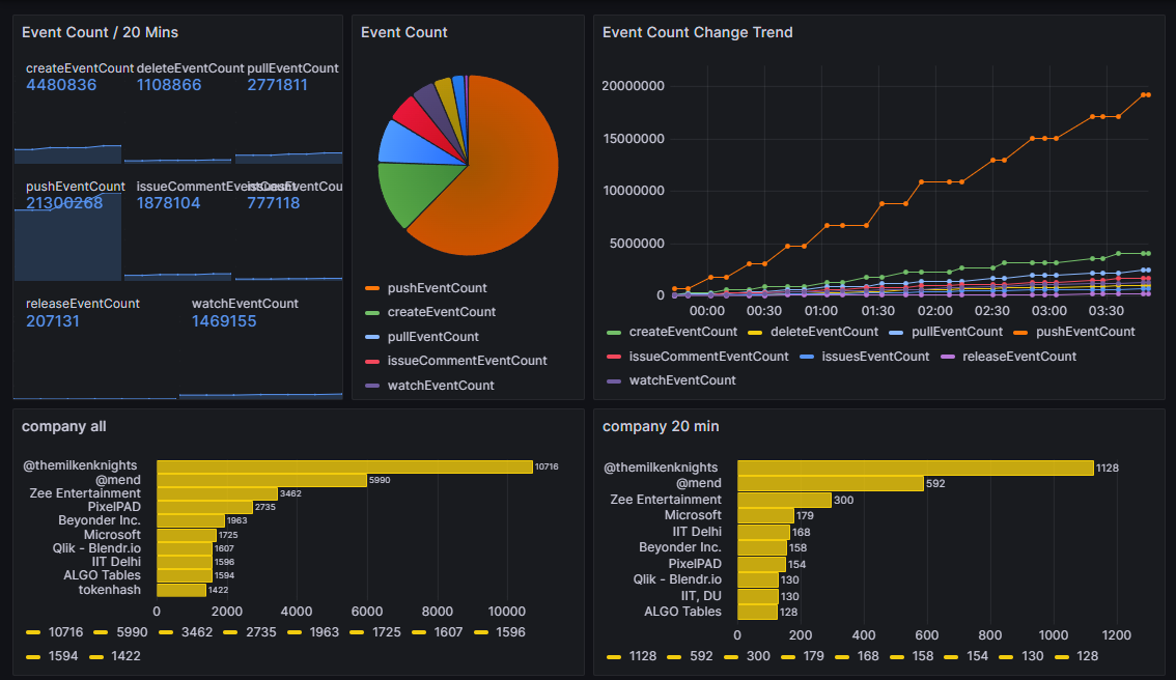
\includegraphics[width=0.48\textwidth]{pic/vis-1.png}
    \caption{Grafana Dashboard}
    \label{fig:grafana-1}
\end{figure}

Figure\ref{fig:grafana-1} shows count of all kinds of event collected in Hive, ratio of different kinds of event, the trend of change of all kinds of events, the top company in the last 10 minutes, and the top company in the whole hive database.




\begin{figure}[H]
    \centering
    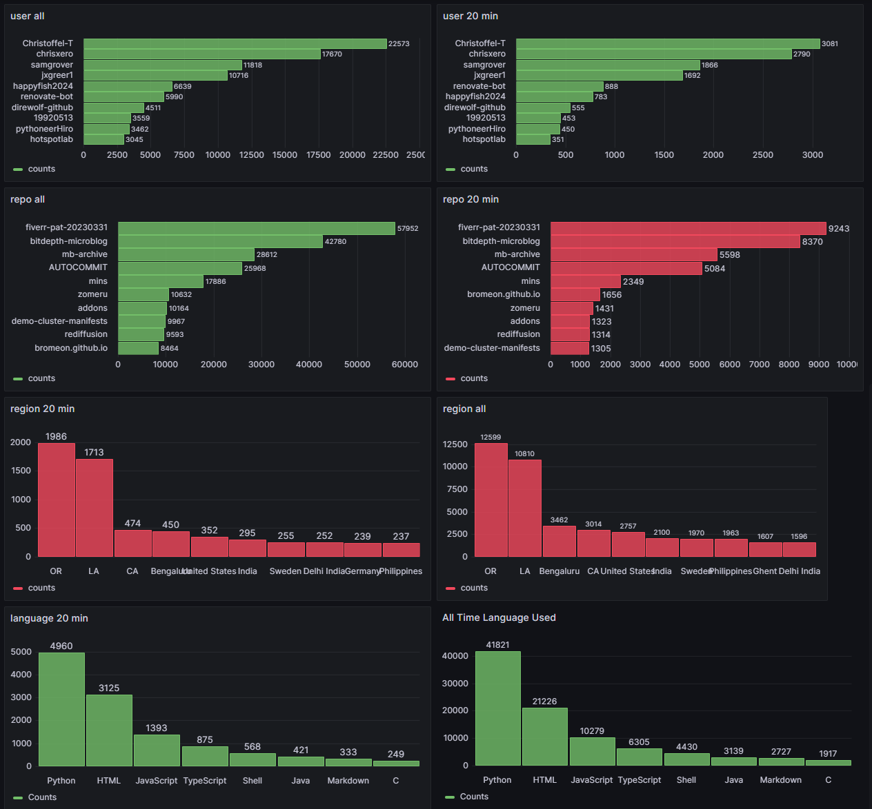
\includegraphics[width=0.48\textwidth]{pic/vis-2.png}
    \caption{Grafana Dashboard}
    \label{fig:grafana-2}
\end{figure}

Figure\ref{fig:grafana-2} show the count of users' event in the whole hive database and in the last past 20 minutes, count of repos' event in the whole hive database and in the last past 20 minutes, the top region in the last 10 minutes, and the top region in the whole hive database

There are indeed some abnormal user and repo with lots of commit in a very short time.
